

\section*{A - Github repository}
\addcontentsline{toc}{chapter}{\protect\numberline{}A - Github repository} 

All simulator code and LaTeX-files used in the thesis provided by the GitHub repositories linked below. Note that both the Comparative Propagation Simulator and GNSS-R Formation Flight Simulator are contained within the \textit{Simulator Repository} link.

\subsection*{Simulator Repository}
% \addcontentsline{toc}{subsection}{\protect\numberline{}Simulator Repository} 
\begin{itemize}
    \item \url{https://github.com/chystad/formation-flight-gnssr-simulator}
\end{itemize}

\subsection*{Master's Thesis LaTeX Repository}
% \addcontentsline{toc}{subsection}{\protect\numberline{}Master's Thesis LaTeX Repository} 
\begin{itemize}
    \item \url{https://github.com/chystad/master-thesis-paper}
\end{itemize}




\clearpage
\section*{B - Simulator Flow Diagrams}
\addcontentsline{toc}{chapter}{\protect\numberline{}B - Simulator Flow Diagrams} 
\subsection*{Comparative Propagation Simulator}
\begin{figure}[H]
    \centering
    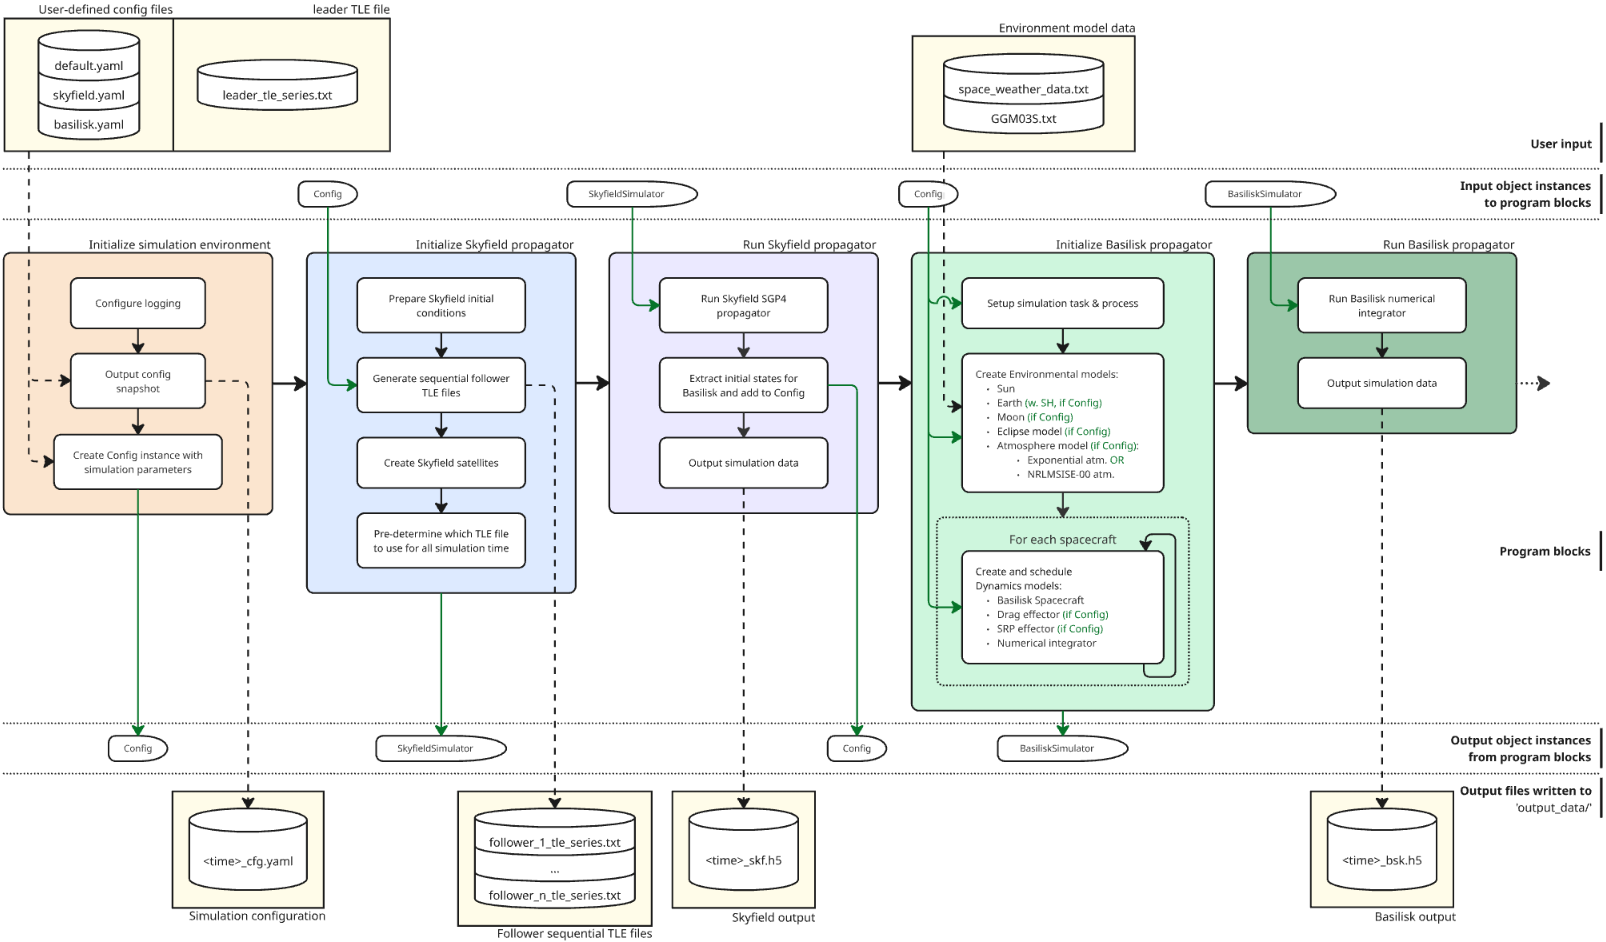
\includegraphics[width=1.3\textwidth, angle=-90]{Figures/04Method/Propagation Accuracy Comparison Simulator Flowchart v2.png}
    \caption{Full size detailed Comparative Propagation Simulator flow diagram}
    \label{fig:full_size_propagator_comp_flow} 
\end{figure}

\subsection*{GNSS-R Formation Flight Simulator}
\begin{figure}[H]
    \centering
    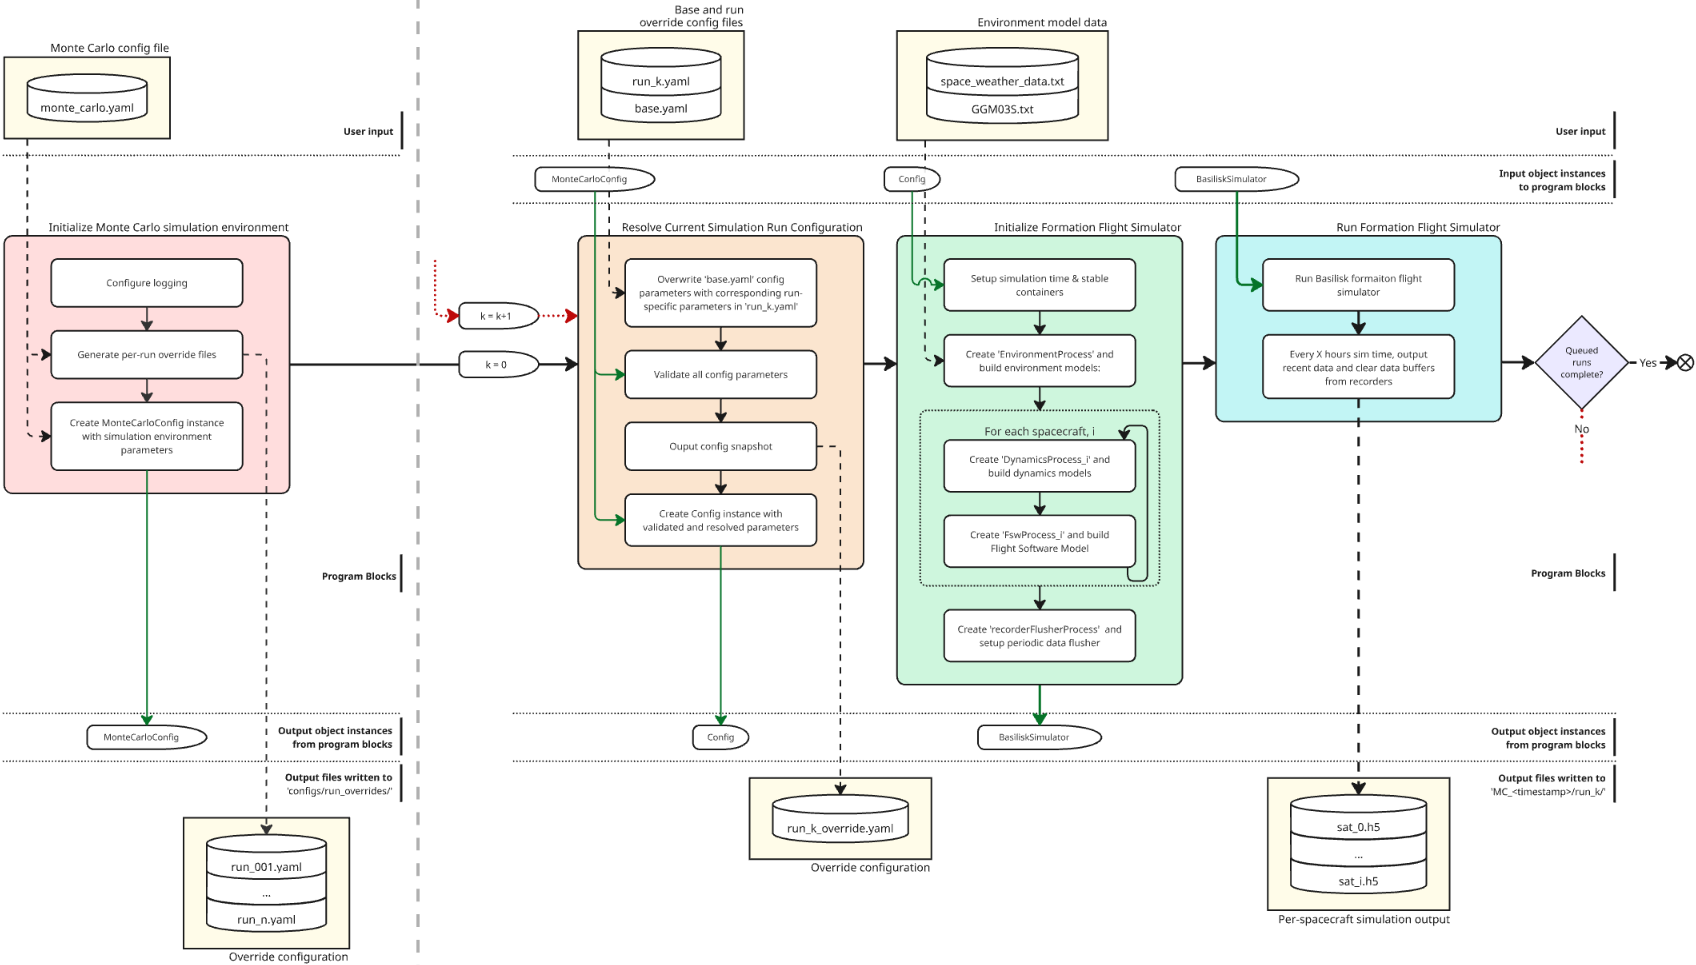
\includegraphics[width=1.4\textwidth, angle=-90]{Figures/04Method/Formation Flight Simulator.png}
    \caption{Full size detailed GNSS-R Formation Flight Simulator flow diagram}
    \label{fig:full_size_formfly_flow} 
\end{figure}


\clearpage
\section*{Simulator Basilisk Process-Task-Model Structure}

\subsection*{Comparative Propagation Simulator}
% Todo

\subsection*{GNSS-R Formation Flight Simulator}
\begin{figure}[htbp]
    \small
    \dirtree{%
    .1 GNSS-R Formation Flight Simulator.
    .2 EnvironmentProcess.
    .3 EnvironmentTask.
    .4 [20] spiceObj.
    .4 [20] eclipseObj.
    .4 [20] groundStation(s).
    .4 [20] atmObj.
    .3 MsisInputUpdaterTask.
    .4 [20] msisInputUpdater.
    .2 DynamicsProcess\_\textless sat\_idx\textgreater.
    .3 DynamicsTask\_\textless sat\_idx\textgreater.
    .4 scObj.
    .4 [20] dragEffector.
    .4 [20] srpEffector.
    .4 [20] solarPanel(s).
    .4 [20] rwEffector.
    .4 [20] thrusterEffector.
    .4 [20] fuelTankEffector.
    .4 [20] battery.
    .4 [20] obcPowerSink.
    .4 [20] rwPower(s).
    .4 [10] recorders.
    .2 FswProcess\_\textless sat\_idx\textgreater.
    .3 FswTask\_\textless sat\_idx\textgreater.
    .4 [20] scheduler.
    .4 [10] recorders.
    .2 RecorderFlusherProcess.
    .3 [20] RecorderFlusherTask.
    .4 [20] recorderFlusher.
    }
    \caption{\hl{TODO: Update and verify after simulator update. Hierarchical process-task-model structure of the GNSS-R formation flight Basilisk simulator. The number in square brackets denote the model priority, where higher priority models are updated first. Same-priority tasks are orderly updated from the top-down within a task. ``\textit{<sat\_idx>}'' represents per-spacecraft processes and tasks.}}
    \label{fig:formfly_process_hierarchy}
\end{figure}

% \clearpage
% \section*{C - Numerical Values}
% \addcontentsline{toc}{chapter}{\protect\numberline{}C - Numerical Values} 

% \section*{Numerical Values for Physical Constants}
% \begin{table}[h!]
% \centering
% \begin{tabular}{c c c}
% \hline
% $Constant$ & $Value$ & $Unit$ \\
% \hline
% $J_0$ & $-1$ & -\\
% $J_1$ & $0$ & -\\
% $J_2$ & $1.08263 \times 10^{-3}$  & -\\
% $J_3$ & $-2.53266 \times 10^{-6}$ & -\\
% $J_4$ & $-1.61962 \times 10^{-6}$ & -\\
% $P_{Sun}$ & $4.578299965 \times 10^{-6}$ & $Ws/m^3$ \\
% $1AU$ & $149597871$ & $km$ \\
% $R$ & $6378136.6$ & $m$ \\
% $H_0$ & $7200$ & $m$ \\
% $\rho_0$ & $1.225$ & $kg/m^3$ \\
% $-$ & $-$ & $-$ \\
% $-$ & $-$ & $-$ \\
% $-$ & $-$ & $-$ \\
% \hline
% \end{tabular}
% \caption{Physical constants and associated numerical value. $J$-terms courtesy of}
% \label{tab:phys_const}
% \end{table}
%%%%%%%%%%%%%%%%%%%%%%%%%%%%%%%%%%%%%%%%%%%%%%%%%%%%%%%%


% \chapter*{B - Sidenote statistics}
% \addcontentsline{toc}{chapter}{\protect\numberline{}B - Sidenote statistics} 

% %For included tables and figures renew the numbering such that they are numbered by the appendix they are attached to and not to the conclusion chapter
% \renewcommand{\thefigure}{B.\arabic{figure}}
% \setcounter{figure}{0}
% \renewcommand{\thetable}{B.\arabic{table}}
% \setcounter{table}{0}


% \section*{\large{B1 - Some random table}}
% \vspace*{1cm}

% Remember to only include one thing per page in the appendices.

% \begin{table}[ht!]
% \centering
%     \begin{tabular}{ m{4cm} m{2.5cm} m{2.5cm} m{2.5cm} } 
%     \toprule
%     \toprule
%     \textbf{Statistic} & \textbf{One} & \textbf{Two}  \\
%     \midrule
%     Count   & 387317    & 283960    \\[1.3ex]
%     Mean    & 130.66    & 134.18    \\[1.3ex]
%     Std     & 248.09    & 230.32    \\[1.3ex]
%     Q1      & 31.00     & 21.00     \\[1.3ex]
%     Median  & 67.00     & 63.00     \\[1.3ex]
%     Q3      & 142.00    & 159.00    \\[1.3ex]
%     Min     & 0.00      & 0.00      \\[1.3ex]
%     Max     & 14519.00  & 14253.00  \\[1.3ex]
%     \bottomrule
%     \bottomrule
%     \end{tabular}
% \caption[Statistics on something]{Table of statistics on some sidenote data.}
% \end{table}


% % Page without title but section title:
% \newpage
% \section*{\large{B2 - Some other random table}}
% \vspace*{1cm}

% \begin{table}[ht!]
% \centering
%     \begin{tabular}{ m{4cm} m{2.5cm} m{2.5cm} m{2.5cm} } 
%     \toprule
%     \toprule
%     \textbf{Statistic} & \textbf{Three} & \textbf{Four}  \\
%     \midrule
%     Count   & 387317    & 283960    \\[1.3ex]
%     Mean    & 130.66    & 134.18    \\[1.3ex]
%     Std     & 248.09    & 230.32    \\[1.3ex]
%     Q1      & 31.00     & 21.00     \\[1.3ex]
%     Median  & 67.00     & 63.00     \\[1.3ex]
%     Q3      & 142.00    & 159.00    \\[1.3ex]
%     Min     & 0.00      & 0.00      \\[1.3ex]
%     Max     & 14519.00  & 14253.00  \\[1.3ex]
%     \bottomrule
%     \bottomrule
%     \end{tabular}
% \caption[Statistics on something else]{Table of statistics on some other sidenote data.}
% \end{table}



% \newpage
% \section*{\large{B3 - Some random figure}}
% \vspace*{1cm}

% \begin{figure}[H]
%   \centering
%   \subfloat[Data set sizes for data X.]
%   {\includegraphics[width=1\textwidth]{Figures/dataset_X.png}}
%   \hfill
%   \subfloat[Data set sizes for data Y.]
%   {\includegraphics[width=1\textwidth]{Figures/dataset_Y.png}}
%   \caption[Data set sizes]{The figures show the data set sizes of X and Y and the proposed cut-off threshold at 10 $\%$ of the mean set size.}
% \end{figure}



%%%%%%%%%%%%%%%%%%%%%%%%%%%%%%%%%%%%%%%%%%%%%%%%%%%%%%%%